\chapter{Oracle APEX HR-1}

\section{Chaitanya Koratamaddi}
 Pada tahun 2005 Chaitanya Koratamaddi manager produk utama yang bekerja pada Oracle dan pada tahun 2010 beliau bertanggung jawab atas manajemen produk APEX di India.
\begin{figure}[!htbp]
    \centering
    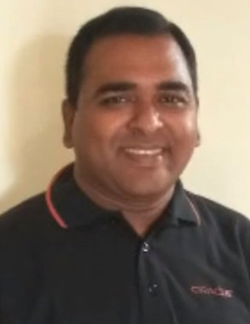
\includegraphics[scale=0.5]{section/gambar_bab1/chaitanya.png}
    \label{penanda}
\end{figure}

\section{Mengembangkan Aplikasi di Enterprise}
Simak dibawah ini jika ingin mengembangka aplikasi pada enterprise.
\begin{enumerate}
    \item Membutuhkan sumber pengembangan khusus dan mahal
    \item Siklus pengembangan aplikasi yang panjang’’
    \item Jaminan simpanan yang besar
    \item Kolaborasi minimal
    \item Bisnis memecahkan masalah dengan tools yang salah
\end{enumerate}

\section{Low Code dan Oracle APEX}
Penggunaan low code pada apex berskala, mudah dijalani, dapat diperpanjang, produktif, dan banyak fungsi pada sedikit kode. Sedangkan oracle APEX adalah low code pengembangan aplikasi kode rendah. Oracle APEX dapat digunakan secara gratis, baik sebagai bagian dari lisensi Oracle Database yang ada atau berjalan dalam produk Oracle Database.

\section{Mengelola Data pada Spreadsheets Menantang}
Mengapa mengelola data pada spreadsheets sangat menantang? Berikut ini adalah penjelasannya.
\begin{enumerate}
    \item Data validation secara manual dan rawan terjadi error
    \item integritas data tidak dapat menjamin dalam keakuratan data pada penggunaan multi-use
    \item Pengamanan data tidak efektif
    \item Data sharing lambat dan susah untuk sharing
\end{enumerate}

\section{Converting Spreadsheet ke Aplikasi Web}
Berikut ini adalah cara meng-convert spreadsheet ke aplikasi web.
\begin{enumerate}
    \item Login ke workspace oracle apex anda
    \item Klik halaman app builder dan arahkan kursor ke from a file
    \item Anda bisa menggunakan drag dan drop file. Format file yang bisa dipilih adalah csv, xlsx, txt, xml, dan json. Atau bisa juga menggunakan copy paste atau memilih sample data movie.
    \item Setelah memilih data, inputlah nama table dari data tersebut.
    
\begin{figure}[!htbp]
    \centering
    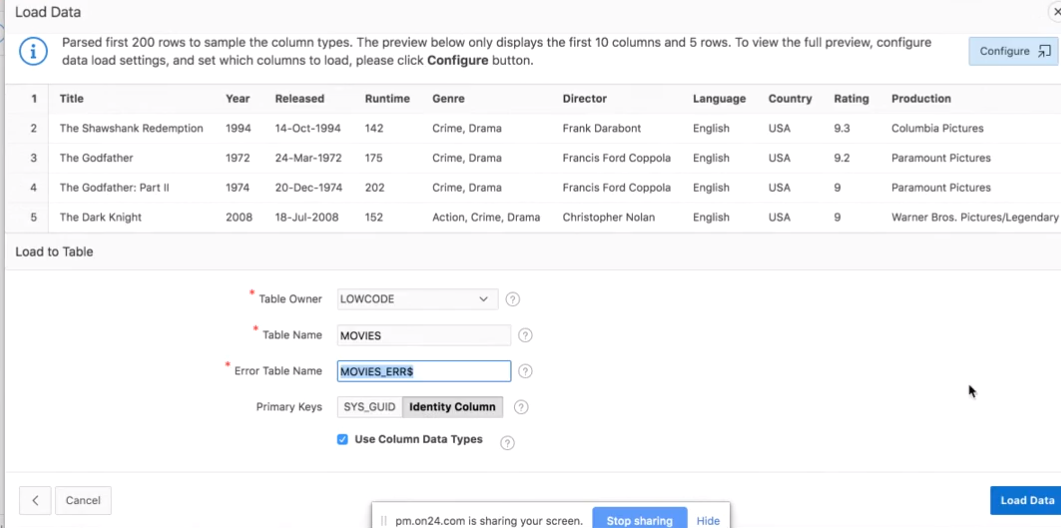
\includegraphics[scale=0.5]{section/gambar_bab1/nama_tabel.png}
    \label{penanda}
\end{figure}
    \item Klik load data dan continue
    \item Beri nama aplikasi yang akan dibuat
    \item Pilh tema dan icon yang akan digunakan
    
\begin{figure}[!htbp]
    \centering
    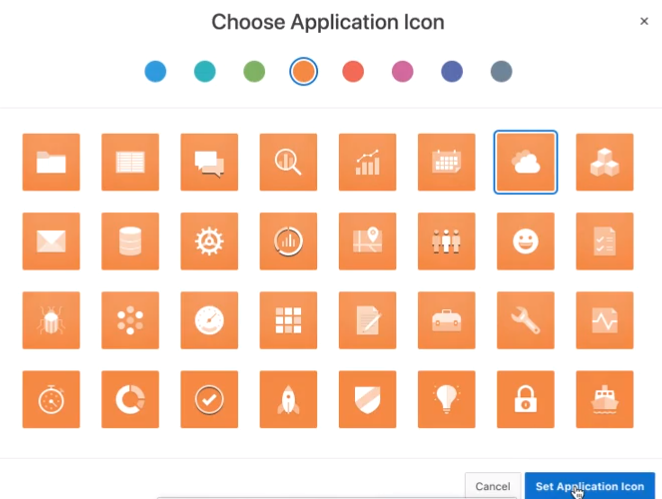
\includegraphics[scale=0.5]{section/gambar_bab1/icon.png}
    \label{penanda}
\end{figure}
    \item {Setelah mengedit dan mengatur semuanya, klik create appliacation}
    \item Untuk melihat aplikasi silahkan sig in terlebih dahulu.
\end{enumerate}


